\documentclass[acmsmall,screen,nonacm]{acmart}

\let\Bbbk\relax
\usepackage{amsmath,amssymb}
\usepackage{amsthm}
\newtheorem{remark}{Remark}
\usepackage{booktabs}
\usepackage{listings}
\usepackage{tikz}
\usetikzlibrary{arrows.meta,positioning,fit,calc}

%% Lean listing style
\definecolor{leankeyword}{RGB}{0,0,255}
\definecolor{leancomment}{RGB}{0,128,0}
\definecolor{leanstring}{RGB}{163,21,21}
\lstdefinelanguage{Lean}{
  morekeywords={theorem,lemma,def,inductive,structure,where,import,open,namespace,end,section,variable,by,have,exact,rcases,intro,apply,sorry,noncomputable,instance,class,abbrev,Type,Prop,Exists,Nonempty},
  sensitive=true,
  morecomment=[l]{--},
  morecomment=[n]{/-}{-/},
  morestring=[b]",
}
\lstset{
  language=Lean,
  basicstyle=\ttfamily\small,
  keywordstyle=\color{leankeyword}\bfseries,
  commentstyle=\color{leancomment}\itshape,
  stringstyle=\color{leanstring},
  breaklines=true,
  columns=flexible,
  showstringspaces=false,
  tabsize=2,
  frame=single,
  numbers=none,
  xleftmargin=1em,
  xrightmargin=1em,
}

\newcommand{\lean}[1]{\lstinline!#1!}
\newcommand{\N}{\mathbb{N}}

\title{Beyond Boolean Intersections: A Typed Boundary Certificate for Causal Graphs}

\author{Lucia Yizi Zhang}
\affiliation{%
  \institution{Shanghai Lixin University of Accounting and Finance}
  \country{China}
}
\email{lucia.zhang.research@outlook.com}
\authorsaddresses{Lucia Yizi Zhang, \href{mailto:lucia.zhang.research@outlook.com}{lucia.zhang.research@outlook.com}, ORCID: 0009-0005-3528-7747}
\orcid{0009-0005-3528-7747}

\setlength{\headheight}{19pt}
\begin{document}

\begin{abstract}
We reframe the interpretability dilemma in artificial intelligence: it is not fundamentally a problem of inscrutability, but of boundary mis-specification. Standard textbook presentations of d-separation decide qualitative path blocking on syntax, but downstream consumers require quantitative information channels. We show that Pearl's abstraction boundary breaks at the moment of type coercion, a failure pattern well known in the programming languages and capability-based security lineage.

We resolve this by defining a typed boundary certificate (\lean{SheafMAGWalk}) and proving its composition soundness in Lean 4. The certificate extends the boolean predicate with stalk-typing, restriction maps, and valuation compatibility. We prove that this four-tuple is exactly the minimal formation data required to turn a causal path into an information channel. The formation rule is accompanied by a certified compilation pipeline from operational trails, an extraction decompiler returning a constructive active-trail witness, and the static-side roundtrip correctness theorem.

Finally, we extend this typed-boundary discipline to the audit of agentic systems, mapping eleven distinct interfaces that each require a channel certificate, shifting the target of safety audit from internal cloud-state to the governance topology.
\end{abstract}
\maketitle

\section{Introduction}\label{sec:intro}

Consider this textbook bug in POPL d-separation. We have the simplest non-trivial directed acyclic graph (DAG): $0 \to 1 \to 2$. Let $X = \{0\}$, $Y = \{1\}$, and $Z = \{0\}$. In Pearl's trail-blocking operational semantics \cite{pearl2009causality}, the one-edge trail $0 \to 1$ has no internal triple, so it cannot be blocked by $Z$. However, in Lauritzen's moralized ancestral-graph separation \cite{lauritzen1996graphical}, the node $0$ (which is in $Z$) is deleted unconditionally, leaving nodes $0$ and $1$ disconnected. The unrestricted equivalence is false.

This concrete discrepancy highlights a broader issue. The resolution is not simply to patch the definition under a disjointness constraint, but to recognize the failure's true nature. As Saltzer and Schroeder observed of operating systems in 1975 \cite{saltzer1975protection}, a system fails at the moment of capability transfer because it lacks a well-defined invariant. Similarly, Pearl's abstraction boundary fails not at causality, but at boundary formation.

We reframe this problem through the lineage of capability-based security and programming language theory. Just as Dijkstra disciplined the \texttt{goto} statement \cite{dijkstra1968goto}, Reynolds established representation independence \cite{reynolds1983types}, Pierce formalized behavioral types \cite{pierce2002types}, and Wadler introduced linear types \cite{wadler1990linear}, we introduce a typed boundary identification for causal graphs.

Our contributions are as follows:
\begin{enumerate}
    \item We localize the failure of causal models to a type mismatch between Pearl's boolean output and downstream theorems' required typed inputs.
    \item We define a typed boundary certificate, \lean{SheafMAGWalk}, to bridge this type-coercion gap.
    \item We prove the composition soundness of these certificates.
    \item We provide a mechanized compiler and decompiler in Lean 4 between trace semantics and graph reachability, proving static-side roundtrip correctness.
    \item We inventory eleven agentic interfaces for industrial AI audit, framing safety around topological capability transfer rather than internal weights.
\end{enumerate}

\section{Pearl Fails at Boundary Formation}\label{sec:boundary}

\subsection{What Pearl Supplies}
Pearl decides one question: \emph{can this path be causally active?} Given a causal DAG $D$ and a conditioning set $Z$, Pearl decides:
\begin{lstlisting}
d-sep(X, Y | Z) : every path p from X to Y in D
                  is blocked under Z by the collider treaty.
\end{lstlisting}
This is a Boolean predicate on the syntactic graph. Nothing more.

\subsection{What Downstream Consumers Need}
The question every downstream consumer---such as NeurIPS-style information-flow certificates, regulatory audits, quantitative information flow (QIF) leakage bounds, or interpretability claims---actually asks is different. To use a cut in any of the following classical theorems, the consumer needs data Pearl never supplies:

\begin{table}[ht]
\centering
\caption{Type mismatch between Pearl's d-separation and consumer requirements.}
\begin{tabular}{ll}
\toprule
Theorem & Argument Pearl does not supply \\
\midrule
Shannon Cut-set Bound & channel object with rate, capacity \\
Conditional DPI & Markov kernel + valuation \\
KKT / Blahut-Arimoto & convex problem on exp-family stalk \\
Counterfactual identification & stalk-level intervention semantics \\
QIF leakage bound & stateLeakage + cutCapacity as numbers \\
\bottomrule
\end{tabular}
\end{table}

Three observed pathologies all surface the same defect:
\begin{enumerate}
    \item \textbf{NeurIPS:} \lstinline!h_cap : I_cut <= C! must be imported as an external premise.
    \item \textbf{Lean QIF:} \lean{condMarkov} must be hypothesized, not derived.
    \item \textbf{POPL d-sep:} \lean{DisjointSets} must be added to repair endpoint-in-$Z$.
\end{enumerate}

Pearl's machinery does not answer quantitative questions. The failure point is precise: it occurs at the moment we ask a qualitative causal separator to act as a quantitative information channel. At the moment of type coercion, there is no legal derivation.

\subsection{The Certificate Object: SheafMAGWalk}
We give a Martin-L\"of-style typed judgment under which a cut is licensed as a channel:
\begin{lstlisting}
D : CausalDAG    F : InformationSheaf D    Z : Set D.V
cut : Set D.V   [path(cut)]   [stalk(cut)]   [res/merge(cut)]   [prob(cut)]
-------------------------------------------------------------------------
                        D, F, Z |- cut : Channel
\end{lstlisting}
Reading: given a causal environment, a stalk-typing environment, a conditioning set, and four local data items, the rule licenses \lean{cut} to appear in the input position of Shannon, DPI, KKT, or QIF theorems.

We name the four-tuple of certificate data \lean{SheafMAGWalk}. It is simultaneously a MAG-style walk on the causal syntax and a section of an information sheaf carrying stalk-level realization data.

\begin{lstlisting}
structure SheafMAGWalk (D : CausalDAG) (F : InformationSheaf D)
                       (Z : Set D.V) (s t : D.V) where
  path         : BaseballPath D s t
  res          : \forall e \in path.edges, F.Stalk e.src \to_p F.Stalk e.tgt
  val          : \forall b \in path.bases, Measure (F.Stalk b)
  val_compat   : pushforward law along non-collider edges
  witness      : \forall c \in path.colliders, ColliderWitness c Z
  merge        : \forall c \in path.colliders, fiber-product on stalks
  merge_compat : collider valuation consistency
\end{lstlisting}

This projects to the syntactic \lean{MAGWalk} (current Lean artifact) by forgetting \lean{(stalk, res, val)}. With this certificate, classical theorems acquire typed signatures:
\begin{lstlisting}
Shannon : (C : Channel, p : InputDist C, k : Code) \to Rate k \le Capacity C
DPI     : (m : MarkovChain X Y Z) \to I(X;Z) \le I(X;Y)
KKT     : (P : ConvexProblem, x : KKT-point P) \to Optimal x
\end{lstlisting}

\subsection{Five Ambient Specializations}
The same formation rule has five canonical specializations under different enriching categories $V$:
\begin{table}[ht]
\centering
\caption{Ambient specializations of the formation rule.}
\begin{tabular}{ll}
\toprule
Ambient & Specialization \\
\midrule
Pearl causal graph & active path with collider witness \\
PL module system & typed interface + capability discharge \\
Probability & sub-$\sigma$-algebra + Markov kernel \\
Sheaf & restriction + gluing axioms \\
QIF & leakage channel + cut capacity \\
\bottomrule
\end{tabular}
\end{table}
These are not metaphors; they are V-instantiations of one judgment.

\section{Soundness of Certificate Composition}\label{sec:soundness}

\subsection{Necessity}
\begin{theorem}[Necessity]
The four fields of \lean{SheafMAGWalk} are exactly the formation data needed to turn a Pearl-style causal path into a channel boundary.
\end{theorem}
Dropping any field loses required structural types: dropping \lean{path} loses the query carrier; dropping \lean{stalk} makes the stalks disconnected; dropping \lean{res}/\lean{merge} removes the restriction maps needed by DPI; dropping \lean{prob} loses quantitative content. Removing any field leaves at least one downstream theorem with an uninhabited argument type.

\subsection{Composition}
\begin{theorem}[Composition]
\lean{SheafMAGWalk} certificates compose along shared endpoints:
given $\text{cert}_1 : \text{SheafMAGWalk}\,F\,D\,Z\,s\,t$
and $\text{cert}_2 : \text{SheafMAGWalk}\,F\,D\,Z\,t\,u$,
there exists $\text{cert} : \text{SheafMAGWalk}\,F\,D\,Z\,s\,u$
with capacity bound $\text{Cap}(\text{cert}) \le \text{Cap}(\text{cert}_1) + \text{Cap}(\text{cert}_2)$
whenever the merge at $t$ is independent.
\end{theorem}
This is the structural law that lets a cut-set bound on a composite agent reduce to a sum of cut-set bounds on its component channels. The independence side-condition is exactly what fixes the per-edge additive-bound pathology.

\subsection{Certificate Checking}
\begin{theorem}[Certificate Checking]
Given an emitted certificate object $c$, each field obligation in \lean{SheafMAGWalk c} is locally checkable by its declared type: path well-typedness, collider-witness membership, restriction/merge typing, and valuation compatibility.
\end{theorem}
This is not a global completeness claim for finding certificates. Search may be delegated to an external compiler; the kernel checks only the certificate it emits. The compiler is outside the trusted kernel.

\subsection{Static-Side Roundtrip}
A typed inverse between original Pearl active traces and generated Lean trace certificates acts as the compiler-correctness theorem for the static side:
\begin{lstlisting}
synth     : ActiveTrace \to TraceSynthesis
decompile : TraceSynthesis \to ActiveTrace

decompile (synth t) = t
synth (decompile c) = c              (on well-typed c)
\end{lstlisting}
This connects to the full d-separation equivalence \lean{dSeparated_iff_dSeparates}.

\section{Internal Mechanism: Compilation Pipeline}\label{sec:pipeline}
The certificate is produced by an explicit compilation pipeline bridging operational semantics and static analysis:
\begin{lstlisting}
Trail
  -[normalize]--------->  BaseballPath           (syntactic)
  -[compressWithFuel]-->  WitnessedPath          (collider treaty eliminated)
  -[realize on F]------>  SheafMAGWalk           (sheaf semantics added)
\end{lstlisting}

\begin{figure}[ht]
\centering
\resizebox{\textwidth}{!}{
\begin{tikzpicture}[
  node distance=1.8cm and 2.4cm,
  every node/.style={align=center, font=\small},
  box/.style={draw, rounded corners, minimum width=2.2cm, minimum height=0.9cm, fill=blue!5},
  arrow/.style={-{Stealth}, thick},
  label/.style={font=\scriptsize\itshape, above, sloped}
]
  % Forward (optimizer)
  \node[box] (trail) {Active trail\\$t : \text{Trail}\,G\,x\,y$};
  \node[box, right=of trail] (bb) {Bayes-ball path\\$p : \text{BayesBallPath}$};
  \node[box, right=of bb] (mag) {MAGWalk\\$w : \text{MAGWalk}\,G\,X\,Y\,Z$};
  \node[box, right=of mag] (reach) {Graph reachability\\$\text{Reachable}_{G'}\,x\,y$};

  \draw[arrow] (trail) -- node[label]{lift} (bb);
  \draw[arrow] (bb) -- node[label]{compress} (mag);
  \draw[arrow] (mag) -- node[label]{embed} (reach);

  % Reverse (decompiler)
  \node[box, below=1.2cm of reach] (rreach) {$\text{Reachable}_{G'}\,x\,y$};
  \node[box, left=of rreach] (rstatic) {StaticRoute\\$r : \text{StaticRoute}$};
  \node[box, left=of rstatic] (ropen) {OpenTrace\\$o : \text{OpenTrace}$};
  \node[box, left=of ropen] (ractive) {ActiveRoute\\$a : \text{ActiveRoute}$};
  \node[box, left=of ractive] (rtrail) {$\exists\,\text{Trail},\;\neg\text{isBlocked}$};

  \draw[arrow, dashed] (rreach) -- node[label]{decompile} (rstatic);
  \draw[arrow, dashed] (rstatic) to [out=110, in=70, looseness=5] node[label]{normalize} (rstatic);
  \draw[arrow, dashed] (rstatic) -- node[label]{compile} (ropen);
  \draw[arrow, dashed] (ropen) -- node[label]{bridge} (ractive);
  \draw[arrow, dashed] (ractive) -- node[label]{realize} (rtrail);

  % Bracket labels
  \node[above=0.3cm of trail, font=\bfseries\small] {Forward: Soundness};
  \node[below=0.3cm of rtrail, font=\bfseries\small] {Reverse: Witness Extraction};
\end{tikzpicture}
}
\caption{The compilation pipeline showing forward and reverse logic.}
\label{fig:pipeline}
\end{figure}

The \textbf{forward direction} lifts an active trail to a \lean{BayesBallPath}. We prove a certified membership theorem ensuring every required state survives deletion of $Z$. This is compressed to a \lean{MAGWalk}.

The \textbf{reverse direction} extracts an active-trail witness from reachability. Reachability yields a \lean{StaticRoute}, which undergoes normalization to eliminate bad colliders via \lean{route_improves_of_bad} (sketched in Appendix~\ref{app:normalization}), decreasing a well-founded measure. A zero-bad \lean{StaticRoute} compiles into an \lean{OpenTrace}, bridging to \lean{ActiveRoute}.

We achieve a zero-sorry verification of this pipeline in Lean 4.

\section{Information-Sheaf Layer}\label{sec:sheaf}
The sheaf is the carrier for stalk data. It provides the internal machinery needed to evaluate information flow on the topological structure.
\begin{lstlisting}
Stalk v       = local information states at v
rho_{v,w}     = restriction / information-flow map for v \le w
mu_v          = valuation on Stalk v
pushforward   : (rho_{v,w})_* mu_v = mu_w
\end{lstlisting}
Stalk-internal geometry lives inside stalks, not on the base poset. Lossiness of restriction is measured by entropy decrease, Fisher pushforward, or finite channel capacity $\sup_\mu I(\mu ; \rho_* \mu) \le C < \infty$. The Lean interface for \lean{InformationSheaf} is outlined in Appendix~\ref{app:sheaf}. This layer is pure machinery: replacing the sheaf with another scheme changes how the certificate is built, but not what it asserts.

\section{Why the Old Boundary Failed: Concrete Examples}\label{sec:failures}

\paragraph{NeurIPS \texttt{h\_cap} as external premise.}
The \lstinline!h_cap : I_cut <= C! premise in existing formalizations is external because \lean{cut} is typed merely as \lean{Set Vertex}. The typed formation rule absorbs this as a discharged sub-obligation within the \lean{SheafMAGWalk} certificate.

\paragraph{\texttt{condMarkov} as external assumption.}
Conditional Markov structure is hypothesized in current formalizations. The formation rule derives it directly: sheaf restriction plus valuation compatibility implement the Markov kernel, and the collider witness implements the conditioning.

\paragraph{Per-edge additive bound pathology.}
Per-edge additive bounds fail because they treat edges as independent channels, ignoring correlations through colliders. The formation rule makes correlation explicit via fiber-merge data, enforcing independent merges as a side-condition for bound summation.

\paragraph{\texttt{DisjointSets}.}
The POPL condition \lean{DisjointSets X Y Z} (preventing an endpoint from being a conditioning variable) is absorbed by the formation rule, which rejects such queries at the path level due to the missing identity restriction $\rho_{X,X} = \text{id}$.

\paragraph{Counter-causality.}
Structures $X \to Y \to Z$ and $X \leftarrow Y \leftarrow Z$ share observational independences but induce different restriction diagrams. Consequently, they yield different \lean{SheafMAGWalk} objects, correctly recognizing directionality without observing it dynamically.

\section{Interface Inventory for Agentic Systems}\label{sec:inventory}
The channel-formation rule scales naturally to systems whose behavior crosses multiple typed boundaries. Industrial LLM agents possess non-trivial information topologies.

\begin{table}[ht]
\centering
\caption{Interface inventory for agentic systems.}
\begin{tabular}{ll}
\toprule
Interface & Description \\
\midrule
token output & user-visible response \\
tool call & external API invocation \\
memory read / write & persistent state across turns \\
scratchpad / chain-of-thought & silent reasoning channel \\
inter-agent message & multi-agent communication \\
retrieval result & RAG / context injection \\
hidden cache & KV cache, prompt cache \\
log boundary & audit trail itself \\
gradient (training time) & data $\to$ weight channel \\
prompt cache & cross-session leakage \\
function trace & call graph as side channel \\
\bottomrule
\end{tabular}
\end{table}
Each row is a cut requiring its own channel-formation certificate. The token-output boundary is the \emph{last} interface, not the only one.

\section{Coverage Gap of Current Methods}\label{sec:gap}

\begin{table}[ht]
\centering
\caption{Coverage gaps in contemporary safety methods.}
\begin{tabular}{lll}
\toprule
Method & Targets & Liftable to certificate? \\
\midrule
RLHF / Constitutional AI & token output & partial (one cut only) \\
Refusal training / Classifiers & token output & partial \\
Sparse autoencoders & activation & not an interface -- cloud \\
Mech interp circuits & weight & not an interface -- cloud \\
Linear probes & activation & descriptive only \\
t-SNE / UMAP & embedding & unliftable (destroys metric) \\
Attention heatmap & activation & descriptive only \\
\bottomrule
\end{tabular}
\end{table}

We identify two profound failure modes:
\begin{enumerate}
    \item \textbf{Coverage failure:} Output-targeted safety methods cover at best one of the eleven interfaces identified in Section~\ref{sec:inventory}.
    \item \textbf{Category failure:} Activation-cloud methods (like sparse autoencoders) are not interface methods. They study internal state rather than typed boundaries. The ``high-dimensional semantic cloud'' interpretability problem is a wrong-boundary artefact, analogous to the dispensability of the luminiferous aether once light's correct frame was identified.
\end{enumerate}

\section{Industrial Implications}\label{sec:industrial}

\subsection{Closed-box Certification}
Behavioural-cut certificates require only an intervention API. Model weights need not be exposed.
\begin{itemize}
\item \textbf{Behavioural:} black-box + intervention API ($\sim$85\% coverage)
\item \textbf{Structural:} + layer activations (additional $\sim$10\%)
\item \textbf{Mechanistic:} + weights (residual $\sim$5\%)
\end{itemize}
This dissolves the regulatory deadlock between white-box audits and intellectual property protection for most compliance use-cases.

\subsection{Precedent}
The channel-formation rule is the AI-agent specialization of capability-based security \cite{levy1984capability,miller2003capability} and the language-based information flow control tradition \cite{denning1976lattice,goguen1982security,myers1997decentralized,sabelfeld2003language}. This shifts the paradigm from a novel AI safety approach to the application of mature PL/OS disciplines to the agentic setting.

\subsection{Multi-cut Audit}
Current auditing frameworks inspect output behaviour and infer everything else. The proposed audit methodology is structural: enumerate interfaces, compute a certificate per interface, and evaluate coverage. Untyped interfaces automatically fail the audit, making safety a property of the governance topology rather than an emergent phenomenon of model weights.

\section{Related Work}\label{sec:related}
\paragraph{Categorical and Topological D-Separation.}
Fritz and Klingler \cite{fritz2023dseparation,fritz2023free} abstracted d-separation using string diagrams in Markov categories. Our approach is complementary: Markov categories provide a generalized measure-theoretic foundation, while our artifact enforces typed boundary identification targeting operational graphs and standard trails.

\paragraph{Mechanized Causal Inference.}
Chancelier, De Lara, and Heymann~(2024) \cite{chancelier2024conditional} and Anna Zhang~(2025) \cite{coqci2025} mechanized d-separation semantic equivalence in Coq. Our contribution differs significantly through the reverse direction witness-extraction pipeline and the typed boundary formation framework provided by our Lean 4 artifact, \lean{CausalQIF}~\cite{causalqif2026}.

\section{Conclusion}\label{sec:conclusion}
We identified a type-coercion gap in standard causal path blocking, defined the typed boundary certificate \lean{SheafMAGWalk}, and proved its composition soundness. By reframing the interpretability dilemma as a type discipline problem, we shift the focus of AI audit from internal weights to topological capability transfers. Our Lean 4 mechanization verifies the foundational pipeline between operational trails and graph reachability without resorting to \lean{sorry} axioms. Future work targets extending the Lean implementation to general measure-theoretic spaces and formalizing numeric probability mass functions to exercise the verification chain end-to-end.

\bibliographystyle{ACM-Reference-Format}
\bibliography{references}

\appendix
\section{Normalization Theorem}\label{app:normalization}
The normalization theorem \lean{route_improves_of_bad} strict-decreases a well-founded measure of bad colliders:
\begin{lstlisting}
theorem route_improves_of_bad
    (w : StaticRouteWitness G X Y Z) (hbad : routeBadCount w \neq 0) :
    \exists w' : StaticRouteWitness G X Y Z,
      routeBadCount w' < routeBadCount w
\end{lstlisting}
The dispatcher extracts the first bad collider, exhibits an ancestral escape into $X$ or $Y$ via helper lemmas (\lean{exists_split}, \lean{ancestor_escape}, \lean{bad_child_survives}, \lean{escape_path_survives}), and replaces one moral jump by zero-cost chain edges.

\section{Endpoint-in-Z Counterexample}\label{app:counterexample}
\begin{lstlisting}
theorem dsep_complete_endpoint_in_Z_counterexample :
    \exists (G : DAG) (X Y Z : Finset \N),
      DAG.dSeparated G X Y Z \wedge \neg dSeparates G X Y Z := by
  refine <chain3, {0}, {1}, {0}, ?_, ?_>
  -- Proof omitted for space, validates topological mismatch
\end{lstlisting}

\section{Dual Witness Upper Bound}\label{app:dualwitness}
\begin{lstlisting}
theorem condMutualInfo_le_of_dual_witness
  -- Bounds the Shannon leakage I(A;B|C) by the KL divergence
  -- between the joint and the factorized witness.
\end{lstlisting}

\section{InformationSheaf Interface}\label{app:sheaf}
\begin{lstlisting}
structure InformationSheaf (I : Type) [Preorder I] where
  Stalk : I \to Type
  res   : {i j : I} \to i \le j \to Stalk i \to Stalk j
  res_id : \forall i, res (le_refl i) = id
  res_comp : \forall {i j k} (hij : i \le j) (hjk : j \le k),
    res (le_trans hij hjk) = fun x => res hjk (res hij x)
\end{lstlisting}

\end{document}
